\section{Methods}\label{sec:methods}

% =========================================================================
%
% EB writes here - this is method but parts of it can also be included in introduction.

\subsection{Vision Transformers} \label{ssec:vit}
\subsubsection{The origin of vision transformers}
In 2017, a novel architecture for deep learning was introduced with the infamous article 
"Attention is all you need" \cite{attention}. This architecture is today known as the 
transformer, and it formed the basis for the current AI wave which includes major 
names such as ChatGPT, Dal-E and AlphaFold 2.

The transformer architecture was originally thought to replace recurrent neural networks (RNN)
as the model of choice for translation of text. The model had several novel ways to train a network,
but the main focus was on the attention mechanism. We will not go into detail on the attention
mechanism here, but it is worth a mention that this concept introduced in 2014 \cite{first_attention}
provides the network with more context for each data point that it tries to predict, which is one
of the aspects that made transformers superior in predicting and later producing full sentences. 

Only three years after the first transformer architecture was introduces, the article 
"An Image is Worth 16x16 Words: Transformers for Image Recognition at Scale" \cite{first_vit}
introduced the first functional transformer trained on images, and it was baptized as a Vision
Transformer (or ViT for short). The authors demonstrate how a ViT outperforms classical 
deep learning methods such as convoultional neural networks (CNN). 

\subsubsection{The function of vision transformers}
A ViT splits an image into even sized, non-overlapping patches, which are then linearly embedded
as token representations. These tokens are then fed into the regular transformer architecture with 
their positional embeddings. The previously mentioned attention mechanism is then used during training
so that the model considered spatial relationships within and between patches. 

The authors of this 
report will not pretend to understand the ViT completely, but we provide the reader with all sources
to fully comprehend this novel architecture, and present the original layout of a ViT in Figure \ref{fig:ViT}

\begin{figure}[H]
    \centering
    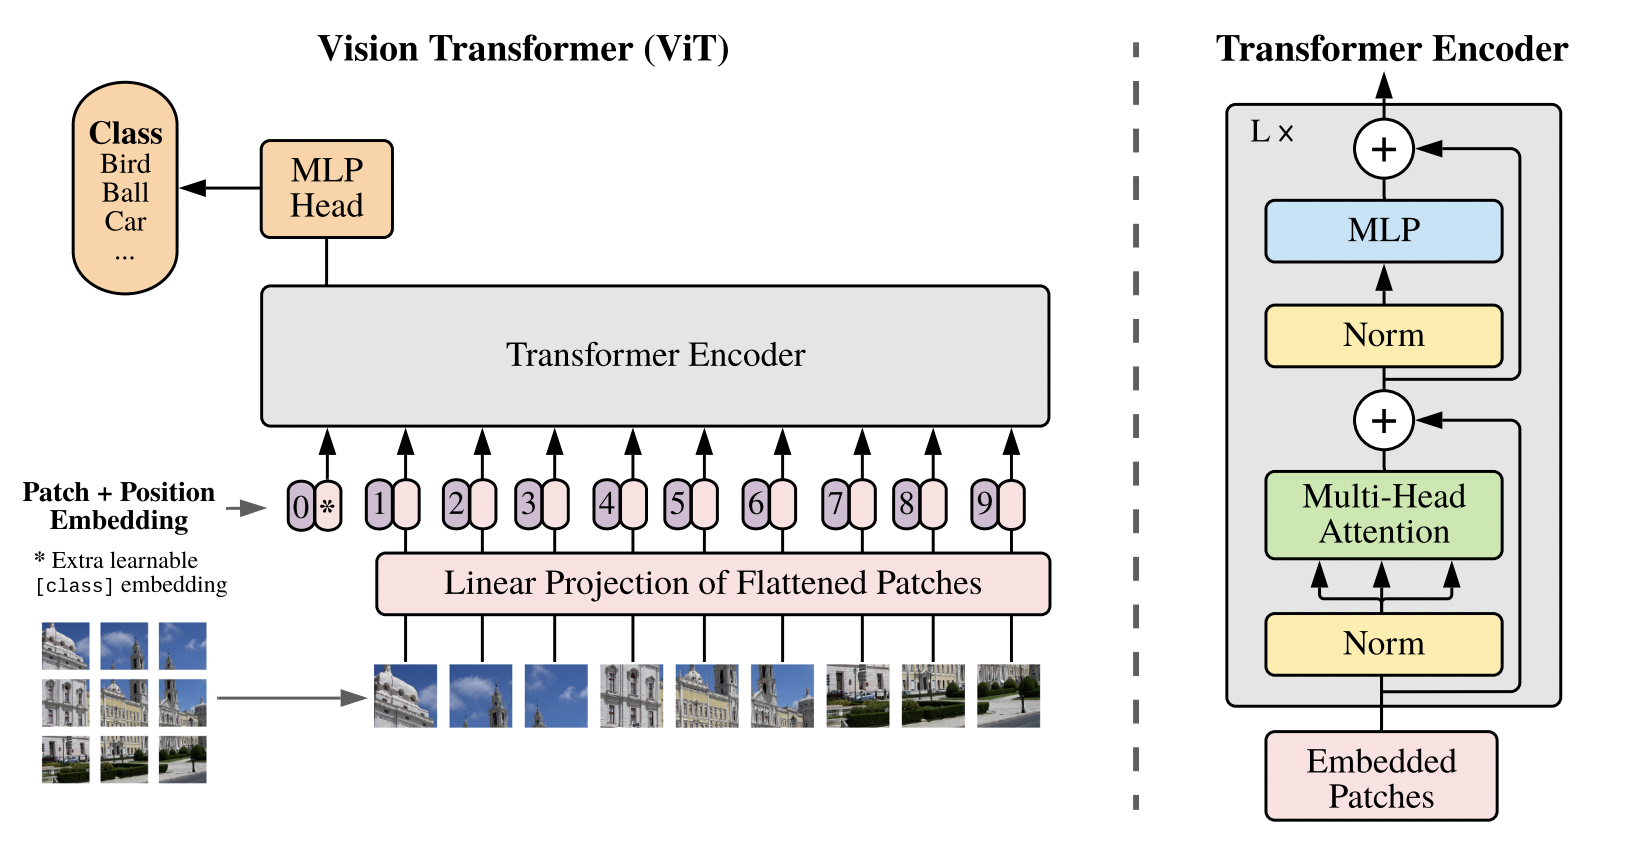
\includegraphics[width=1.1\linewidth]{examples/tests_eb/figs/vit.png}
    \caption{Vision Transformer layout as presented from it's original paper by Dosovitskiy et. al \cite{first_vit}}
    \label{fig:ViT}
\end{figure}

\subsubsection{Self-\textbf{di}stillation with \textbf{no} labels (Meta's \textbf{DINO})} \label{sssec:dino}
The first DINO was introduced by Facebook (now Meta) shortly after the original ViT was proposed \cite{dino1}, as a self-supervised computer vision method inspired by the "Bootstrap your own latent"-method of self-supervision \cite{byol}. The authors found that DINO works exceptionally well with ViT architechtures, and their model achieved 80.1\% top-1 on ImageNet in linear evaluation.  

The self-\textbf{di}stillation aspect refers to a teacher-student interaction, where a teacher model looks into global augmented crops of an image and the student model looks into both smaller (local), augmented crops and global, augmented crops of the same image. The goal is that both the student and the teacher gives us the same feature representation of the different crops, essentially teaching the model that minor deviations in size and color should still fall into the same representation. A simple figure from the original article is shown in Figure \ref{fig:dino}.

\begin{figure}[H]
    \centering
    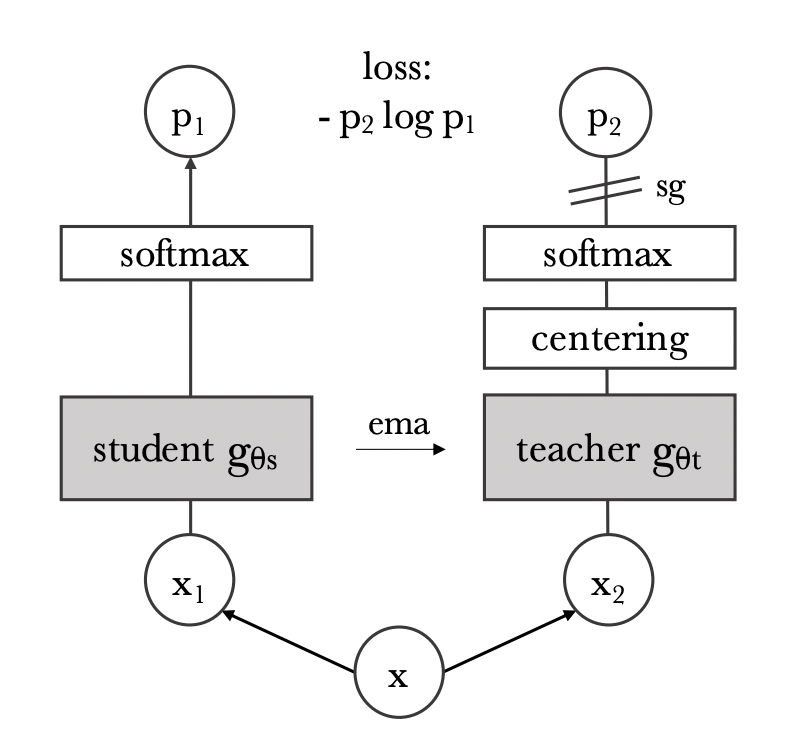
\includegraphics[width=0.7\linewidth]{examples/tests_eb/figs/dino.png}
    \caption{Student-Teacher interactions as presented in original DINO article \cite{dino1}.}
    \label{fig:dino}
\end{figure}

We will not give a full explanation of the DINO functionality, but it is important to note that it is self-supervised and has shown exceptional performance on extracting a set of features to represent an image. 

This performance has since increased with Meta's newest release of the updated \textbf{DINOv2} \cite{dino2} from january 2024, which they offer as an open source, pre-trained ViT model of 1B parameters. The model produces a set of visual features and has been trained on LVD-142M, meaning 142 million images. The authors themselves make the claim that the newest DINOv2 does not require any fine tuning, and we've therefore chosen to go for their reccomended approach. 


%
% =========================================================================

% =========================================================================
%
% Janita writes here
%
% =========================================================================

% =========================================================================
%
% Even writes here
%
% =========================================================================